%!TEX root = paper.tex
%%%%%%%%%%%%%%%%%%%%%%%%%%%%%%%%%%%%%%%%%%%%%%%%%%%%%%%%%%%%%%%%%%%%%%%%%%%%%%%%
\section{The Crowdsensing Mobile App Prototype}
\label{sec:prototype}

A community crowdsensing service faces several challenges in its task of gathering and processing the data before making it available in a concise and easy-to-understand visualized way. The goal for the gathering portion is to measure in an automated, non-interactive fashion in order to be non-intrusive to the participants as well as reach a larger audience. This allows for a larger geographical coverage of the project service quality values while simultaneously being more conservative with the available resources. The implementation of these aspects is discussed in this section.


%%%%%%%%%%%%%%%%%%%%%%%%%%%%%%%%%%%%%%%%%%%%%%%%%%%%%%%%%%%%%%%%%%%%%%%%%%%%%%%%
\subsection{The Issue of Bandwidth Measurements}
\label{sec:BWest}

The most important directly measurable network \gls{QoS} metric for a \acrshort{TCP}-based %(and thus ensuring an in-order, lossless transmission, with the potential caveat of head-of-line blocking when packets are lost)
 video streaming service is arguably the achievable goodput of this flow%(which can also be influenced by the \gls{RTT}, especially for delay-based \acrshort{TCP} congestion control variants)
. Typically, this would be calculated by downloading a file from a remote location and dividing its size by the time it took to transmit it. This is inherently an average value over a certain time period, which makes it tricky to pinpoint it to specific spatial coordinates when this is employed during a mobile crowdsensing campaign.

Furthermore, it is especially crucial to not waste the participants monthly data caps solely on the estimation of video streaming quality. In some countries the monthly contractual data caps are set extremely low. For example, in Germany postpaid contracts with a data cap of \SI{1}{\giga\byte} currently cost a monthly fee of around \SI{25}{\EUR}. On the other hand, only measuring the user's actually watched video streams would provide an insufficient amount of samples for providing accurate data for mobile networks. This means that in order to widen the possible audience, direct throughput measurements of streaming services are out of the question. Our measurement prototype attempts to solve these issues by implementing several bandwidth estimation methods, which trade a loss of accuracy for much less data and time usage. The rest of this section aims to evaluate if the precision of these methods is sufficient for the \gls{QoE} crowdsensing endeavor.


\subsubsection{Bandwidth Estimation Methods: Basics and Variants}

These bandwidth estimators can be roughly divided into two different categories. Approaches from the first category, namely \textit{Cross-Traffic Estimation}, actively send a small amount of probe packets with fixed inter-packet times. On the bottleneck link the timing of these are altered through network throughput limitations as well as traffic from other sources, from which the bandwidth can then be calculated. One well-known representative of this category is Packet Pair~\cite{Bolot:1993:EPD:167954.166265,749288}. The second set of approaches, termed \textit{Self-Induced Congestion}, relies also on active probes, but here they are meant to briefly congest the network themselves in order to observe the resulting path characteristics. Packet Train~\cite{Jain02pathload:a} is one such variant implemented here.

It should be noted that some methods require the presence of an actively sending server under the control of the measurement client with the possible benefit of a better measurement accuracy, making it unfeasible to measure public services like YouTube with them. Packet Pair is one of them. However, it is also usually possible to circumvent this requirement by exploiting known properties of \acrshort{TCP}. For example, some approaches \cite{saroiu2002sprobe,Chakravarty08linkwidth:a} force the transmission of \gls{TCP} RST packets through specifically crafted \gls{TCP} SYN packets and then time the interaction.
% This has not yet been fully implemented in the prototype client but is envisioned to do so in the future.


%%%%%%%%%%%%%%%%%%%%%%%%%%%%%%%%%%%%%%%%%%%%%%%%%%%%%%%%%%%%%%%%%%%%%%%%%%%%%%%%
\subsection{Prototype and Estimator Evaluation}

To evaluate the feasibility of these methods as well as to establish a foundation for the participatory crowdsensing aspects a prototype was set up. This was realized as a Java-based Android application. 
%During development we recognized that the networking functionality exposed through the Android SDK might be insufficient to read and write arbitrary packets to sockets with the necessary temporal precision required to acquire meaningful results from the estimation methods. Therefore, the part that handles the raw networking sockets has been outsourced to C-code attached by \gls{JNI} through Android's \gls{NDK}.
Both the prototype, with the bandwidth estimation and data collection and upload methods\footnote{\url{https://github.com/mas-ude/bw-estimation-App}}, and the  server-side components required for some of the bandwidth estimation methods\footnote{\url{https://github.com/Nobodi/Bandwith-Estimation}}, are available online.

\begin{figure}[!t]
	\centering
	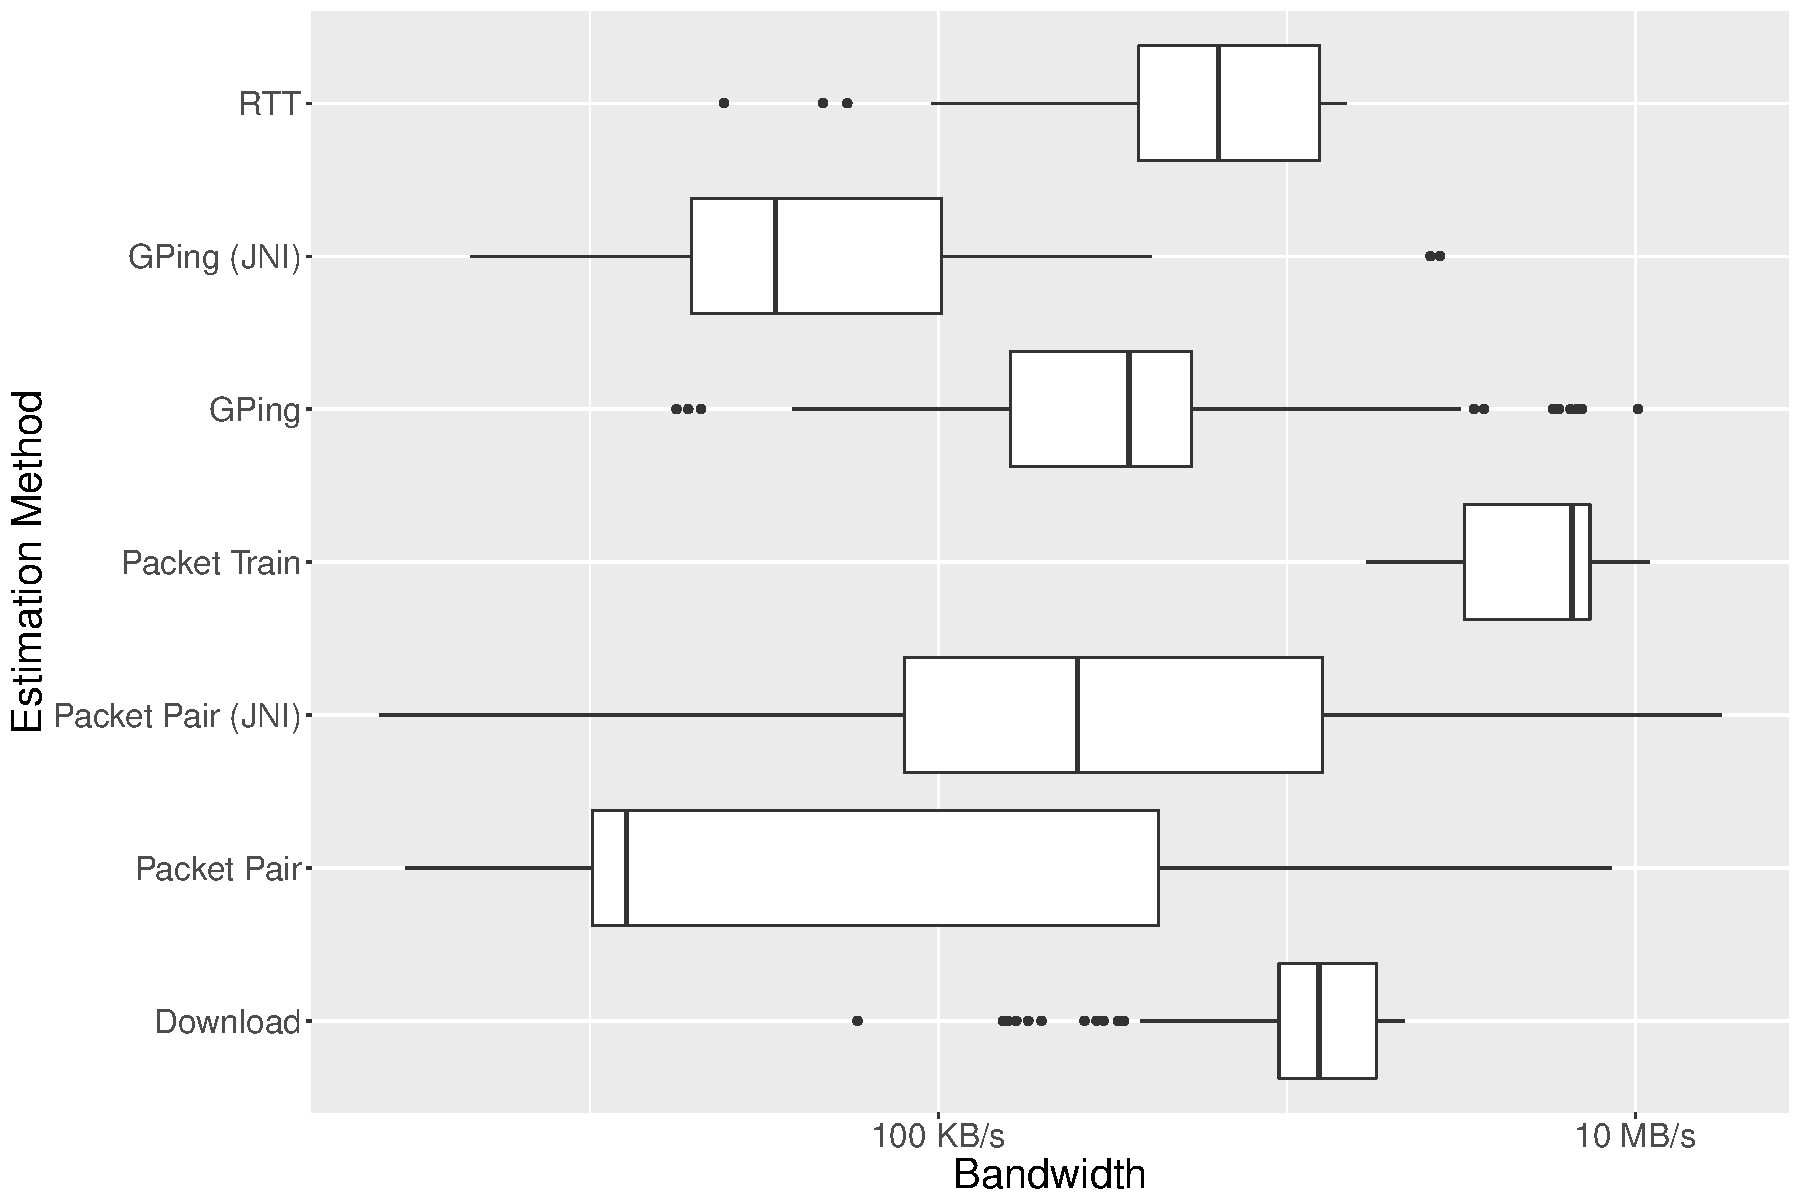
\includegraphics[width = 1.0\columnwidth]{images/BWest-boxplots.pdf}
	\caption{Boxplots of the various tested throughput estimation methods in the evaluation scenario. Entries denoted with JNI use system-level packet and timing facilities in an attempt to improve accuracy.}
\label{fig:boxplots}
\end{figure}

Evaluating the addressed estimation methods is not as straight-forward as one might expect in a mobile environment due to the many factors that can influence the results to a small or large degree. To compensate for these factors this evaluation was conducted in a more controlled setting. All evaluations ran on a single mobile phone, an \textit{LG G3}, and were fixed to a single location to avoid varying radio conditions. Similarly, all corresponding runs were closely grouped together to ensure reasonable temporal coupling. These runs were conducted in five-minute intervals for roughly one day. Various methods described in the literature (as mentioned above) were tested in comparison to the results from simple download tests with a large file. The method dubbed `RTT' is a variant of download, but is using very small files, transferred from a controlled server environment, to calculate its throughput estimate, making it potentially less accurate.

\begin{table}[!t]
\caption{Data usage of the estimation methods.}
\label{tab:datausage}
	\begin{tabu}{XSS}
		\toprule
		 & {\textbf{Used Volume (\si{\kilo\byte})}} & {\textbf{Duration (\si{\second})}} \\
		 \midrule
		\textbf{Download} & 10240 & 9.42 \\
		\textbf{RTT} & 256 & 0.36 \\
		\textbf{Packet Pair} & 6 & 0.37 \\
		\textbf{GPing} & 2.5 & 0.14 \\
		\textbf{Packet Train} & 437 & 0.89 \\ % 437 -- 6035 
		\bottomrule
	\end{tabu}
\end{table}

Figure~\ref{fig:boxplots} depicts the results attained from this scenario. The inter-quartile ranges of the accumulated samples reveal, with every method except RTT, rather large deviations from the download results. The root cause is unclear in this limited evaluation, but this kind of estimation error does not come entirely unexpected due to the aforementioned temporal instability of mobile networks, even in a static location. All of the applied methods generally expect certain network properties to hold that are unfortunately only loosely applicable to mobile networks, with their strong form of a signaling plane. On approach to remedy this situation is to apply an adjustment factor to the individual methods if the offset to the download results proves to be stable enough in a wider range of scenarios.

However, one other benefit is clear when looking at the data and time used during the measurements in Table~\ref{tab:datausage}. The intended goal of being more resource-friendly in order to target a wider audience can be easily fulfilled with these methods, especially with the single-pair approaches Packet Pair and GPing, allowing for more frequent probing and thus more coverage on a crowdsensed community \gls{QoE} map.





% GPing~\cite{6918916} does something similar albeit with differently sized packets.

% \begin{figure}[!t]
% 	\centering
% 	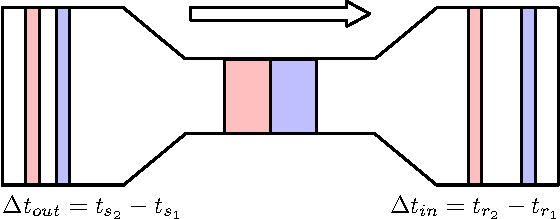
\includegraphics[width=1.0\columnwidth]{images/packetpair.pdf}
% 	\caption{Packet Pair scheme (adopted from \cite{Lai01nettimer:a}.}
% \label{fig:packetpair}
% \end{figure}



% \begin{figure}[!t]
% 	\centering
% 	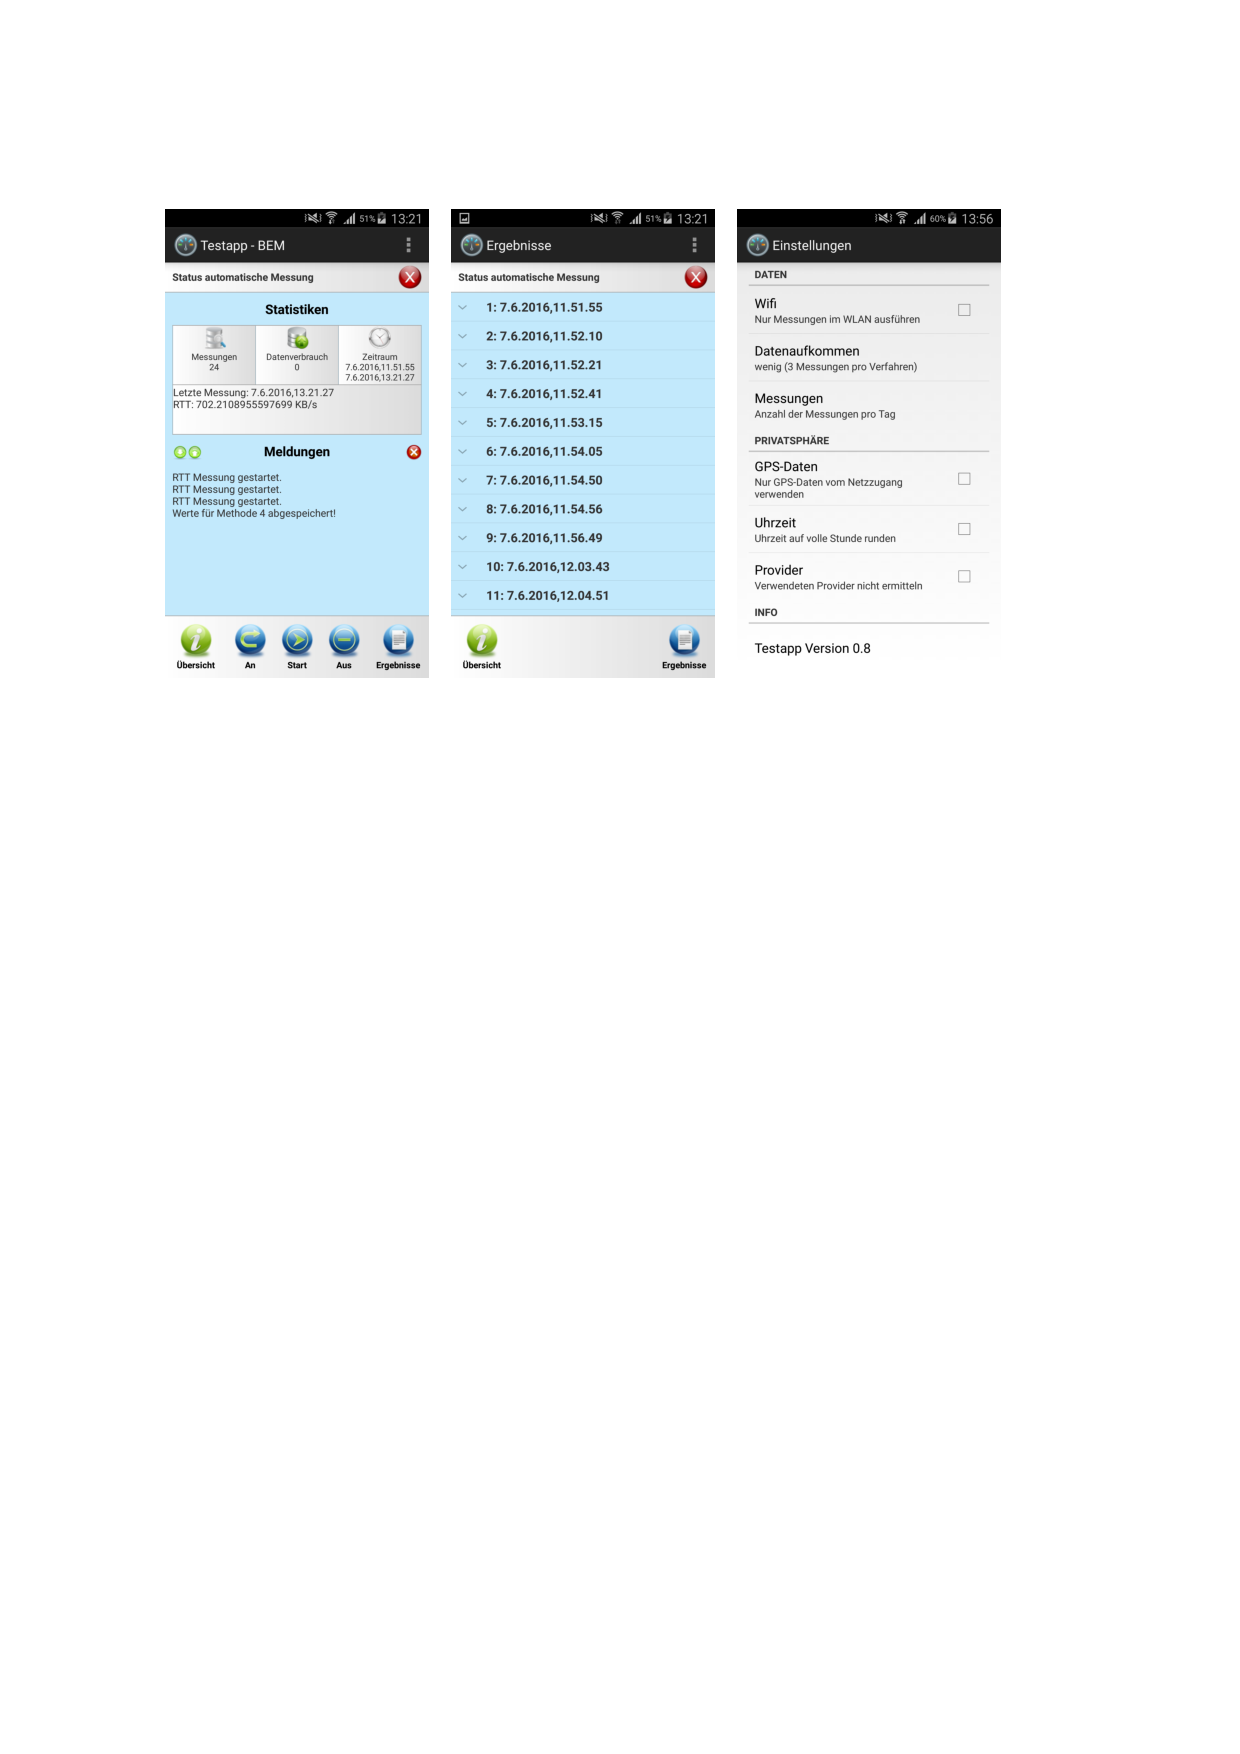
\includegraphics[width=1.0\columnwidth]{images/screenshots.pdf}
% 	\caption{[PH] Screenshots of the bandwidth testing prototype.}
% \label{fig:prototype-screens}
% \end{figure}




%%%%%%%%%%%%%%%%%%%%%%%%%%%%%%%%%%%%%%%%%%%%%%%%%%%%%%%%%%%%%%%%%%%%%%%%%%%%%%%%
%\subsection{Estimation Method Evaluation}

% \begin{figure}[!t]
% 	\centering
% 	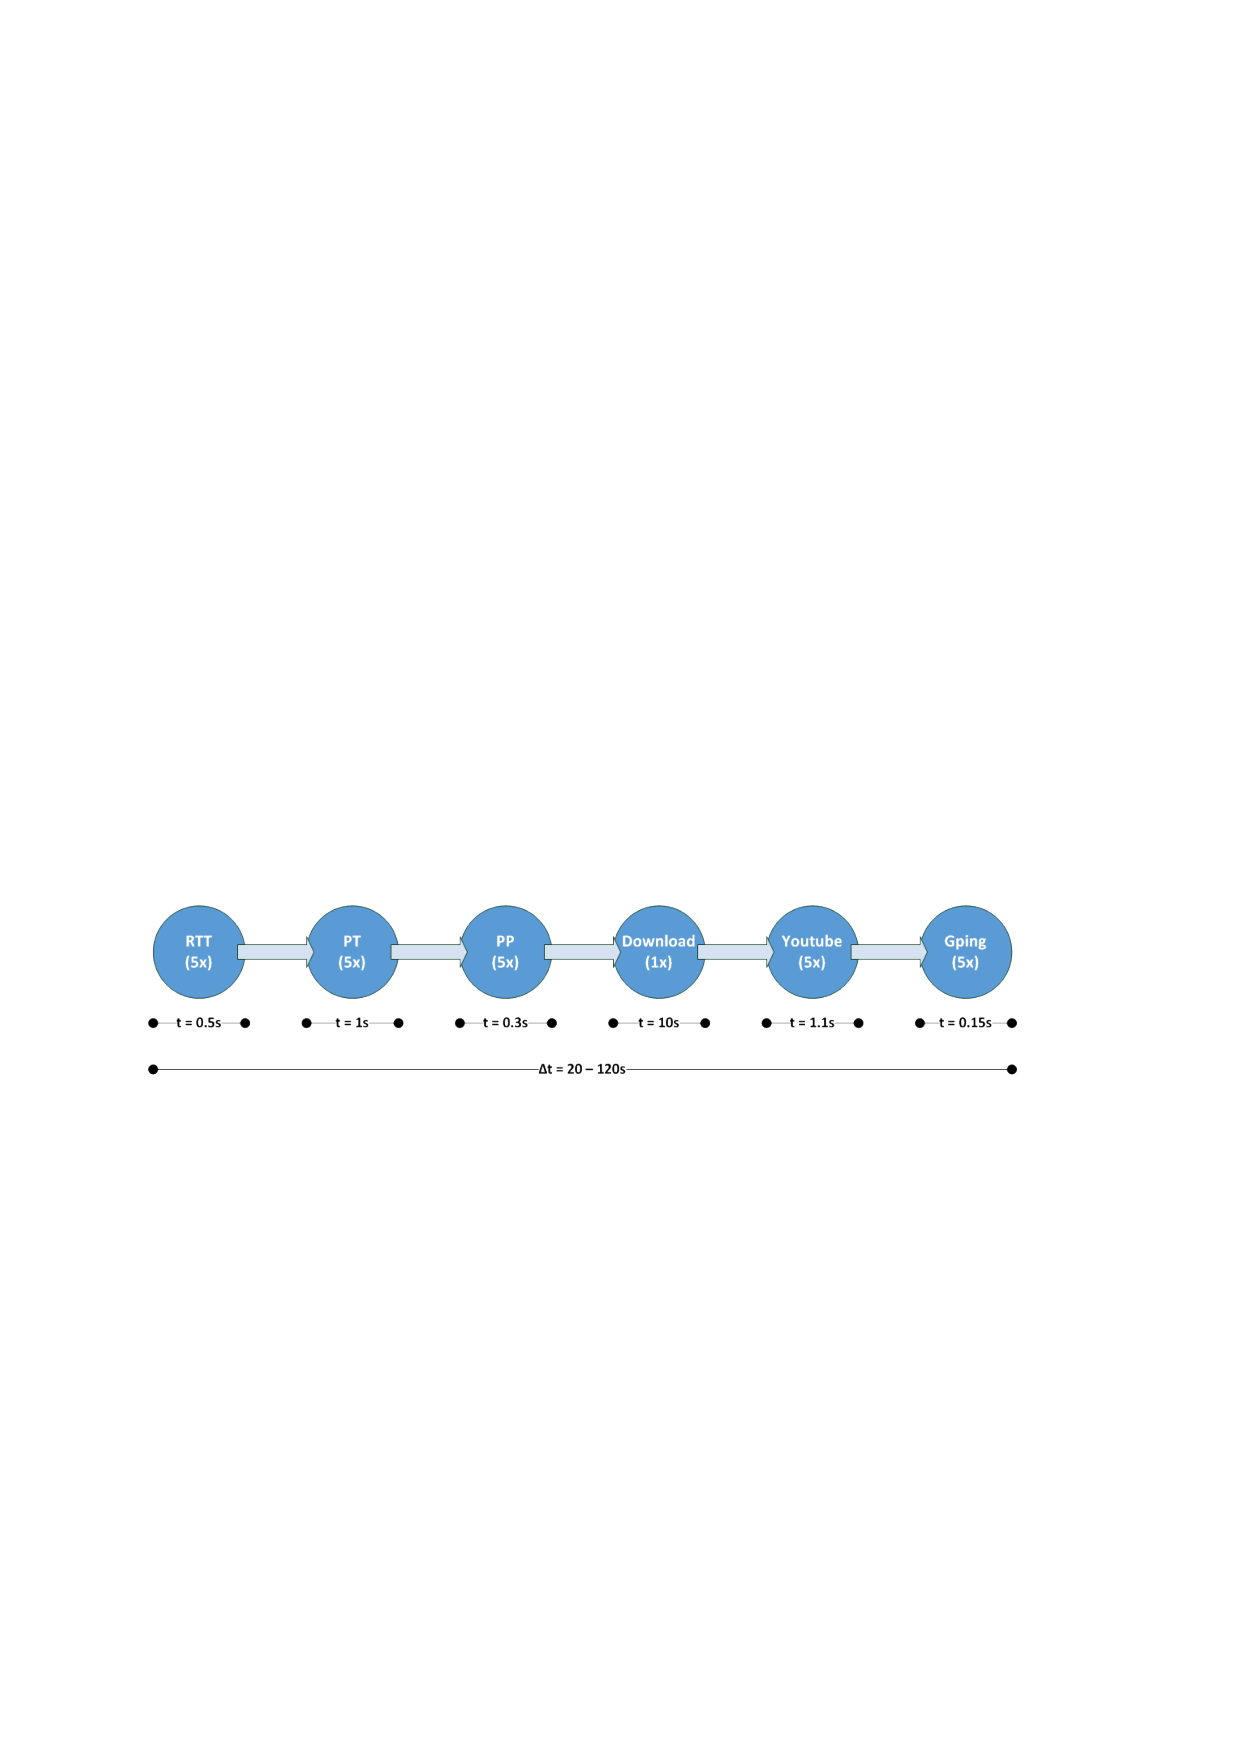
\includegraphics[width=1.0\columnwidth]{images/eval-methodology.pdf}
% 	\caption{Sketch of one bandwidth estimation method measurement cycle.}
% \label{fig:mcycle}
% \end{figure}






% \begin{table}
% \caption{Data usage of the methods.}
% \label{tab:data}
% 	\begin{tabu}{XSSSS}
% 		\toprule
% 		 & {Average} & {SD} & {Used Volume} & {Duration} \\
% 		 \midrule
% 		Download & 1320.94 & 473.35 & 10240 & 9.42 \\
% 		RTT & 1086.83 & 432.56 & 256 & 0.36 \\
% 		Packet Pair & 1560.52 & 5742.10 & 6 & 0.37 \\
% 		GPing & 857.03 & 1456.42 & 2.5 & 0.14 \\
% 		Packet Train & 5399.98 & 2034.44 & 437 & 0.89 \\ % 437 -- 6035 
% 		\bottomrule
% 	\end{tabu}
% \end{table}